\documentclass[a4paper]{article}
%\usepackage[singlespacing]{setspace}
\usepackage[onehalfspacing]{setspace}
%\usepackage[doublespacing]{setspace}
\usepackage{geometry} % Required for adjusting page dimensions and margins
\usepackage{amsmath,amsfonts,stmaryrd,amssymb,mathtools,dsfont} % Math packages
\usepackage{tabularx}
\usepackage{colortbl}
\usepackage{listings}
\usepackage{amsmath}
\usepackage{amssymb}
\usepackage{amsthm}
\usepackage{enumerate}
\usepackage{enumitem}
\usepackage{subcaption}
\usepackage{float}
\usepackage[table,xcdraw]{xcolor}
\usepackage{tikz-qtree}
\usepackage{forest}
\usepackage{pgfplots}
\usepackage{changepage,titlesec,fancyhdr} % For styling Header and Titles
\pagestyle{fancy}
\renewcommand{\headrulewidth}{0.5pt} % Linienbreite anpassen, falls gewünscht
\renewcommand{\headrule}{
    \makebox[\textwidth]{\rule{1.0\textwidth}{0.5pt}} 
}
\usepackage{amsmath}
\pagestyle{fancy}
\usepackage{diagbox}
\usepackage{xfrac}

\usepackage{enumerate} % Custom item numbers for enumerations

\usepackage[ruled]{algorithm2e} % Algorithms

\usepackage[framemethod=tikz]{mdframed} % Allows defining custom boxed/framed environments

\usepackage{listings} % File listings, with syntax highlighting
\lstset{
	basicstyle=\ttfamily, % Typeset listings in monospace font
}

\usepackage[ddmmyyyy]{datetime}


\geometry{
	paper=a4paper, % Paper size, change to letterpaper for US letter size
	top=3cm, % Top margin
	bottom=3cm, % Bottom margin
	left=2.5cm, % Left margin
	right=2.5cm, % Right margin
	headheight=25pt, % Header height
	footskip=1.5cm, % Space from the bottom margin to the baseline of the footer
	headsep=1cm, % Space from the top margin to the baseline of the header
	%showframe, % Uncomment to show how the type block is set on the page
}
\lstset{
  language=C++,
  basicstyle=\ttfamily\small,
  numbers=left,
  numberstyle=\tiny,
  stepnumber=1,
  numbersep=5pt,
  backgroundcolor=\color{white},
  showspaces=false,
  showstringspaces=false,
  showtabs=false,
  frame=single,
  rulecolor=\color{black},
  tabsize=2,
  captionpos=b,
  breaklines=true,
  breakatwhitespace=false,
  keywordstyle=\color{blue},
  commentstyle=\color{purple},
  stringstyle=\color{red}
}
\lhead{Badan, 7418190\\Kneifel, 8071554}
\chead{\bfseries{\vspace{0.5\baselineskip}HL-BPR Praktikum SS25\\Blatt 02}}
\rhead{Wolf, 8019440\\Werner, 7987847}
\fancyheadoffset[R]{0cm}

\begin{document}
\section{Exercise 1.1}
General Ideas and Plans:
\begin{itemize}
    \item using Fliplist to store which cells need to be inverted (column and line indices of a cell)
    \item using nested vectors to store our cells (game-board)
    \item computing a 3x3 neighbor grid for each cell before applying the given rules while respecting edge wrapping (edges and corners connect to the opposite side of the game-board)
    \item custom library for pleasant user interface
\end{itemize}
\begin{figure}[H]
    \centering
    \includegraphics[width=1\linewidth]{classdiagram.png}
    \caption{UML Classdiagram}
\end{figure}
\clearpage
\section{Exercise 1.2}
\subsection{Evolve}
This is our main game loop, here we have defined the given game Rules via the following nested if-statements 
\begin{lstlisting}[caption={"Game Rules"}]
// Rules of the game as stated on Wikipedia
if (board[j][i] == true) {
    if (liveCellCount < 2) {
        flipList.push_back(make_tuple(j, i)); // (x, y)
    } else if (liveCellCount > 3) {
        flipList.push_back(make_tuple(j, i));
    }
} else {
    if (liveCellCount == 3) {
        flipList.push_back(make_tuple(j, i));
    }
}
\end{lstlisting}
After Deciding which cells need to be Flipped (killed or born) we then also Flip them (invert their current state)
\begin{lstlisting}[caption={"Changing cell States"}]
// The flipping of the flipList elems
for (tuple<int, int> coords : flipList) {
    int j = get<0>(coords);
    int i = get<1>(coords);

    board[j][i] = !board[j][i]; //inverting bool
}

secondTolastFlipList = lastFlipList;
lastFlipList = flipList;
flipList.clear();

print();
\end{lstlisting}
\clearpage
\subsection{load}
This Functions loads a World from a file, it reads the worlds dimensions from the first two lines and saves the rest into a nested vector, it also checks if the file is valid by making sure that it only reads 1s and 0s.
\begin{lstlisting}[caption={main loop of the load function}]
string line;
//Iterator to iterate through the matrix (to address the sublists)
auto sublist_It = matrix.begin();
while (getline(file, line) && sublist_It !=matrix.end()) {
    //skipping the first 2 lines as those only serve to save the dimesnions
    linenumb ++;
    if (linenumb<=1) continue;
    stringstream str_s(line);
    int val;
    // this loop checks if only 1s and 0s are present in the document (except the frist 2 lines)
    while (str_s>>val){
        if(val!=0 && val!=1) {
            cerr << "Error only 1s and 0s allowed";
            return{};
        }
        sublist_It ->push_back(val!=0); //adding the bools into the sublists
    
    }
++sublist_It; // iterates through sublists

}
\end{lstlisting}
\clearpage
\subsection{save}
The save Function saves the current state of the game as a txt file, for this each subvector of the nested vector is saved as a line in the file after the dimensions of our board/matrix are detected and saved as the first two lines in the file.
\begin{lstlisting}
ofstream outfile(saveName);
if (!outfile) {
    return 1;
}
else {
    outfile << board.size() << endl; // adding the x dimension
    outfile << board.begin()-> size()<<endl; // adding the y dimesnion
}
// writing the elements from the list to the file
for (const auto& sublist : board) {
    for (bool elem : sublist) {
        outfile << elem << " ";
    }
    outfile << endl;
}
\end{lstlisting}
\subsection{isstable}
This Function checks if any changes have been made since the last round of the game, it does this by comparing the current fliplist last and or second to last one. If they match up perfectly then the game is stable, if not then a flase is returned.
\begin{lstlisting}
bool is_stable() {
if (flipList == lastFlipList) {
return true;
} 
else if (flipList == secondTolastFlipList) {
return true;
}
return false;
}
\end{lstlisting}
\clearpage
\subsection{print}
This function prints out our current board state using unicode symbols to make it more readable.
\begin{lstlisting}
ofstream outfile(saveName);
if (!outfile) {
    return 1;
}
else {
    outfile << board.size() << endl; // adding the x dimension
    outfile << board.begin()-> size()<<endl; // adding the y dimesnion
}
// writing the elements from the list to the file
for (const auto& sublist : board) {
    for (bool elem : sublist) {
        outfile << elem << " ";
    }
    outfile << endl;
}
\end{lstlisting}
\subsection{Additional Functions}
\subsubsection{getNeighboredCells}
This function is used to create a 3x3 grid of all the neighbors of a given cell with the given cell being at the center of the grid (position 1,1), this grid is used in another function (getNeighborMatchCount) to figure out how many living or dead neighbours a cell has.
\begin{lstlisting}
vector<vector<bool>> getNeighboredCells(int coordX, int coordY) {
    vector<vector<bool>> neighborGrid(3, std::vector<bool>(3, false));

    for (int dimYCounter = -1; dimYCounter <= 1; ++dimYCounter) {
        for (int dimXCounter = -1; dimXCounter <= 1; ++dimXCounter) {
            // Wrap around using modulo
            int ni = (static_cast<int>(coordY) + dimYCounter + dimY) % dimY;
            int nj = (static_cast<int>(coordX) + dimXCounter + dimX) % dimX;

            neighborGrid[dimYCounter + 1][dimXCounter + 1] = board[ni][nj];
        }
    }
    return neighborGrid;
}
\end{lstlisting}
\clearpage
\subsubsection{getNeighborMatchCount}
This functions counts how many neigbours ofa cell match a state that is being asked for (either dead or alive) if our cell also matches the state in question we subtract the number of matched cells by one as not to count it as a neighbor of itself.
\begin{lstlisting}
// this func counts how many neighbors match a state that we are looking for (dead or alive)
int getNeighborMatchCount(vector<vector<bool>> neighborGrid, bool state) {
    int matchCount = 0;

    for (const vector<bool>& row : neighborGrid) {
        for (bool cell : row) {
            if (cell == state) {
                matchCount += 1;
            }
        }
    }
    // subtracting matchcount by one if our cell matches the state in question
    if (neighborGrid[1][1] == state) {
        matchCount -= 1;
    }
    return matchCount;
}
\end{lstlisting}
\subsubsection{getTerminalSize}
With this function we try to check the Dimensions of our Terminal, if this fails we ask the used to manually input the Dimensions.
\begin{lstlisting}
void getTerminalSize() {
    // Try to get terminal dimensions
    if (ioctl(STDOUT_FILENO, TIOCGWINSZ, &w) == -1) {
        std::cerr << "Unable to determine terminal size. Please enter dimensions manually:\n";
        std::cout << "Terminal width (characters): ";
        std::cin >> terminalDimX;
        std::cout << "Terminal height (rows): ";
        std::cin >> terminalDimY;
    } else {
        terminalDimX = w.ws_col;
        terminalDimY = w.ws_row;
    }
}

\end{lstlisting}
\clearpage
\subsection{exercise 1.4}
DISCLAIMER: Because the run time for 2000 generations was too high, we used 10 generations. The real times would be approx. times 200.

The times for compiling with the help of the DEBUG mode:
\begin{itemize}
    \item Flag O0:  3m56.856s
    \item Flag O1:  4m58.583s
    \item Flag O2:  5m22.436s
    \item Flag O3:  5m20.077s
\end{itemize}
The times for compiling with the help of the RELEASE mode:
\begin{itemize}
    \item Flag O0:  3m48.844s
    \item Flag O3:  5m27.411s
\end{itemize}
Normally one would think that by going up in the optimization level, the run time would reduce. In that particular programm that does not seem to be the case.
The flag O0 does not increase runtime, as there are not any optimizations.

The flag O1 decreases efficiency by deleting variables that are not used or factoring terms into into simpler terms. But trying to optimize source code that cannot be optimized, can even increase the runtime. That is the case here.

The flag O2 and O3 optimize the programm by a much larger margin, but these optimizations cannot be used here, as the code should be written for such an optimization. Flag O2 tries to decrease runtime by combining variables or rolling out loops. Flag O3 tries to increase the runtime in a more aggressive manner, but those optimizations are not usable in this source code and can even increase the runtime.

The difference in Flag O0 and O3 (in both modes) are huge. The compiler tries to optimize code by using different techniques (examples above). But before the compiler can optimize anything, the source code should be optimized for the higher level of flags. \\ \\
The times above are run on a slower computer. Trying the program on a computer much faster gives us this time:
\begin{lstlisting}[caption={"test on a different machine
"}]
❯ g++ -O0 -g main-test.cpp -o main-test && ./main-test
Loop took 451 milliseconds.
❯ g++ -O1 -g main-test.cpp -o main-test && ./main-test
Loop took 149 milliseconds.
❯ g++ -O2 -g main-test.cpp -o main-test && ./main-test
Loop took 145 milliseconds.
❯ g++ -O3 -g main-test.cpp -o main-test && ./main-test
Loop took 139 milliseconds.
❯ g++ -O4 -g main-test.cpp -o main-test && ./main-test
Loop took 134 milliseconds.
\end{lstlisting}

The times calculated here are more in line with what we imagined in the context of the optimization. The computer used here, or rather the compiler that was run on it, was better able to use the optimizations of the flags O1, O2 and O3. The optimizations include, for example, the removal of unused code, constant calculation or vectorization (in flags O2 and O3).


\section*{Exercise 1.5}

We cut/extended (with zeros) our matrix so that the desired dimensions are maintained. Inside of the directory are the files, with the other dimensions, which can be run.
\begin{center}
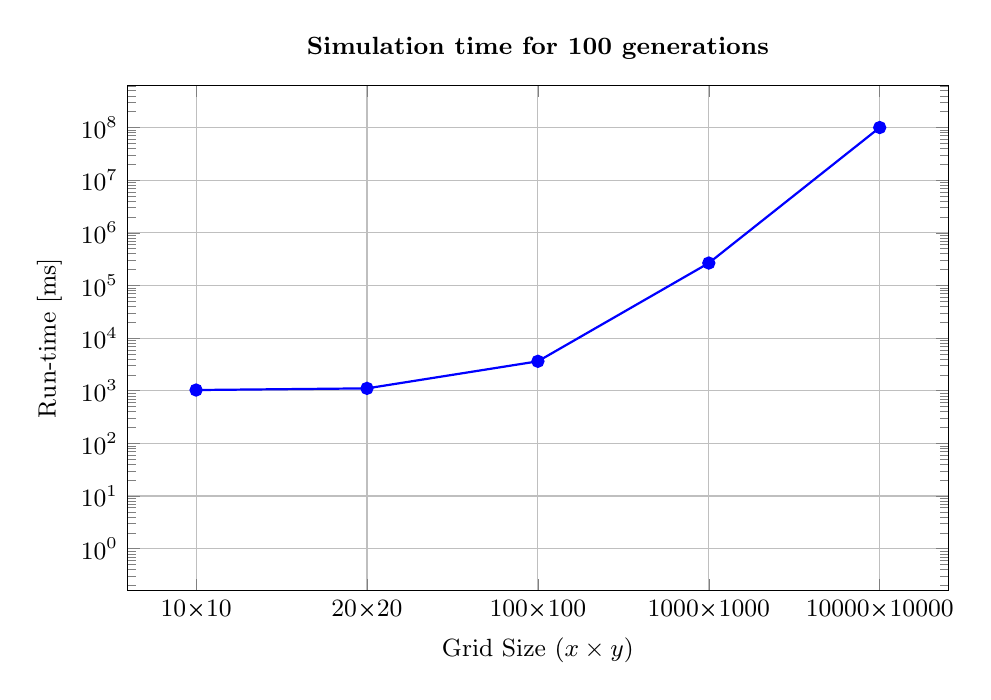
\begin{tikzpicture}
\begin{axis}[
    width=12cm,
    height=8cm,
    xlabel={Grid Size ($x \times y$)},
    ylabel={Run-time [ms]},
    title={Simulation time for 100 generations},
    xtick=data,
    xticklabels={{10×10}, {20×20}, {100×100}, {1000×1000}, {10000×10000}},
    ymode=log, 
    log basis y=10,
    ymin=1,
    ymax=100000000,
    grid=major,
    enlargelimits=0.1,
    tick label style={font=\small},
    label style={font=\small},
    title style={font=\small\bfseries},
]
\addplot[
    mark=*,
    color=blue,
    thick
] coordinates {
    (1, 1032)
    (2, 1110)
    (3, 3627)
    (4, 266628)
    (5, 100000000)
};
\end{axis}
\end{tikzpicture}
\end{center}

The runtime of the 10,000x10,000 matrix took so long that we only used an estimated value. (approx. 24 h) 
The estimated time is calculated from how long the program was busy with the 1000x1000 matrix times 100, i.e. approx. 100,000,000 ms = 27 h.


\end{document}